\documentclass[a4paper,12pt]{article}
\usepackage{amsmath,amssymb,amsfonts,amsthm}
\usepackage{tikz}
\usepackage[utf8x]{inputenc}
\usepackage[T2A]{fontenc} 
\usepackage[russian]{babel}
\usepackage{cmap} 
\usepackage{ gensymb }
% Так ссылки в PDF будут активны
\usepackage[unicode]{hyperref}
\usepackage{ textcomp }
\usepackage{indentfirst}
\usepackage[version=3]{mhchem}

% вы сможете вставлять картинки командой \includegraphics[width=0.7\textwidth]{ИМЯ ФАЙЛА}
% получается подключать, как минимум, файлы .pdf, .jpg, .png.
\usepackage{graphicx}
% Если вы хотите явно указать поля:
\usepackage[margin=1in]{geometry}
% Или если вы хотите задать поля менее явно (чем больше DIV, тем больше места под текст):
% \usepackage[DIV=10]{typearea}

\usepackage{fancyhdr}

\newcommand{\bbR}{\mathbb R}%теперь вместо длинной команды \mathbb R (множество вещественных чисел) можно писать короткую запись \bbR. Вместо \bbR вы можете вписать любую строчку букв, которая начинается с '\'.
\newcommand{\eps}{\varepsilon}
\newcommand{\bbN}{\mathbb N}
\newcommand{\dif}{\mathrm{d}}

\newtheorem{Def}{Определение}


\pagestyle{fancy}
\makeatletter % сделать "@" "буквой", а не "спецсимволом" - можно использовать "служебные" команды, содержащие @ в названии
\fancyhead[L]{\footnotesize }%Это будет написано вверху страницы слева
\fancyhead[R]{\footnotesize ФУПМ МФТИ}
\fancyfoot[L]{\footnotesize \@author}%имя автора будет написано внизу страницы слева
\fancyfoot[R]{\thepage}%номер страницы —- внизу справа
\fancyfoot[C]{}%по центру внизу страницы пусто

\renewcommand{\maketitle}{%
	\noindent{\bfseries\scshape\large\@title\ \mdseries\upshape}\par
	\noindent {\large\itshape\@author}
	\vskip 2ex}
\makeatother
\def\dd#1#2{\frac{\partial#1}{\partial#2}}


\title{4.2 \\ Исследование энергетического спектра $\beta$-частиц и определение их максимальной энергии при помощи магнитного спектрометра}
\author{Северилов Павел, 674} 
\date{08 октября 2018 г.}

\begin{document}
	
	\maketitle
	\section{Теоретическое введение}
		Бета-распад это самопроизвольное преваращение ядер, при котором их массовове число не изменяется, а заряд изменяется на единицу. В данной работе мы будем иметь дело с электронным распадом:
		\begin{equation}
		    _{Z}^{A}X \rightarrow _{Z+1}^{A}X + e^{-} + \widetilde{\nu}
		\end{equation}
		Освобождающаяся в результате распада энергия делится между исходным ядром, электроном и нейтрино. При этом доля энергии, уносимая ядром крайне мала, так что вся энергия делится между нейтрино и электроном. Поэтому электроны могут иметь любую энергию от нулевой до некоторой макимальной энергии, высвобождаемой при распаде.
		
		Вероятность $\dif\omega$ того, что электрон вылетит с имульсом $\dif^3p$, а нейтрино с импульсом $\dif^3k$ равна произведению этих дифференциалов, но мы должны учесть также закон сохранения энергии.
		\begin{equation}
		    E_e - E - ck = 0
		\end{equation}
		Энергия электрона связана с импульсом обычным образом:
		\begin{equation}
		    E = c\sqrt{p^2 + m^2c^2} -mc^2
		\end{equation}
		Таким образом, вероятность $\dif\omega$ принимает вид:
		\begin{equation}
		    \dif\omega = D\delta(E_e-E-ck)\dif^3p\dif^3k = D\delta(E_e-E-ck)p^2\dif pk^2\dif k\dif\Omega_e\dif\Omega_{\widetilde{\nu}}
		\end{equation}
		D можно считать с хорошей точностью константой. В этом случае можно проинтегрировать по всем углам и по абсолютному значению импульса нейтрино. В этом случае $\delta$-функция исчезнет, а $ck$ всюду заменится на $E_e-E$. После умножения на полное число распадов выражение примет вид:
		\begin{equation}
		    \dif N = \frac{16\pi^2N_0}{c^2} D p^2\left(E_e-E\right)^2\dif p
		\end{equation}
		В нерелятивистском случае выражение упрощается и принимает вид:
		\begin{equation}
			\frac{\dif N}{\dif E} \simeq \sqrt{E}(E_e - E)^2
		\end{equation} 
		\begin{figure}[h!]
			\centering
			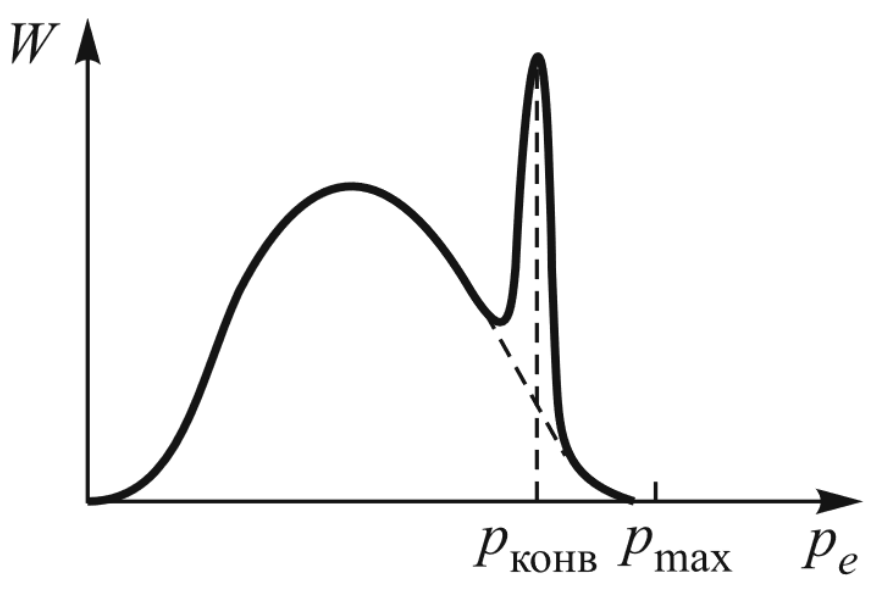
\includegraphics[width=0.6\linewidth]{pic1}
			\caption{Форма спектра $\beta$-частиц при разрешенных переходах}
		\end{figure}
		\section{Экспериментальная установка}
		Энергия определяется с помощью $\beta$-спектрометров. В работе используется магнитный спектрометр с короткой линзой.
		\begin{figure}
			\centering
			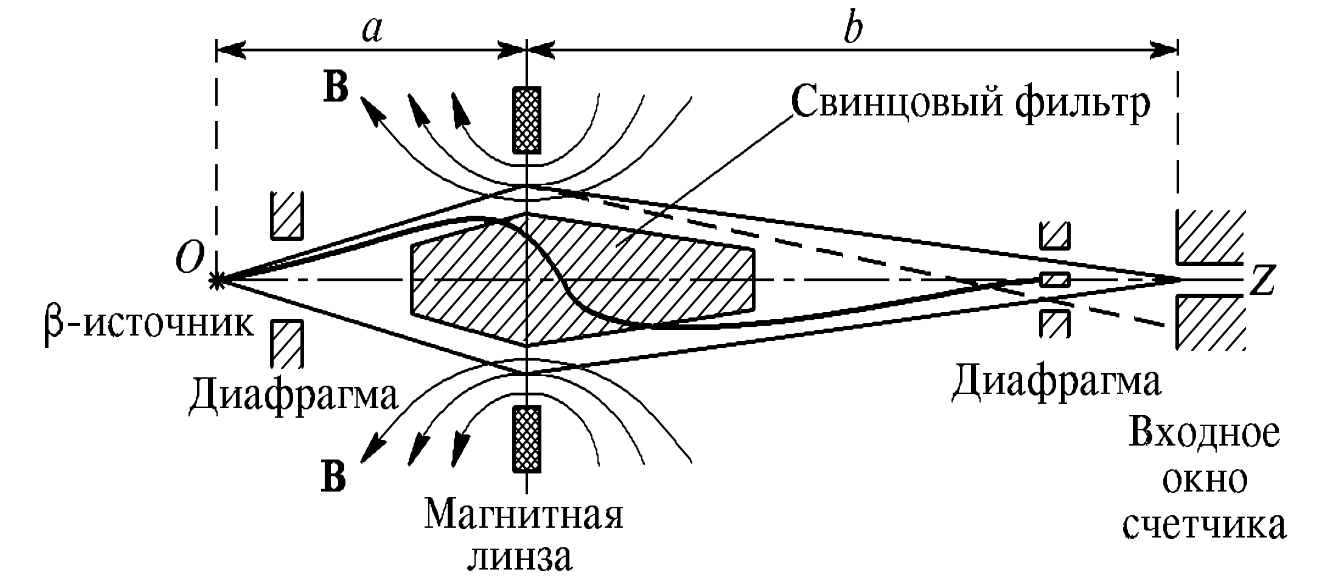
\includegraphics[width=0.8\linewidth]{pic2}
			\caption{Схема $\beta$-спектрометра с короткой линзой}
		\end{figure}
		Как показывает расчет, для заряженных частиц тонкая катушка эквивалентна линзе:
		\begin{equation}
			\frac{1}{f} \simeq \frac{I^2}{p_e^2}
		\end{equation}
		При заданной силе тока на входное окно счетчика собираются электроны с определенным импульсом.

    \section{Экспериментальные данные}
    Подготовили установку к работе согласно пунктам 1 − 4 лабника и запустили ПЭВМ в режим проведения измерения спектра. Измерения проводим по 80 секунд, изменяя ток магнитной линзы через 0.2 ампера. В результате чего получаем с учётом фона график
    
    \begin{table}[h!]
\centering
\caption{Экспериментальные данные}
\label{my-label}
\begin{tabular}{|l|l|l|l|l|l|}
\hline
$J, A$&	$N, 1/s$&	$N-N_p, 1/s$&	$p, kEv/s$&	$T, kEv$&	$mkFermi$ \\ \hline
0.00&	0.537&	0&	0.0&	0.0&	0.00 \\ \hline
0.20&	0.662&	0.125&	47.2&	2.2&	1090.2827 \\ \hline
0.40&	0.750&	0.75&	94.5&	8.7&	502.3433 \\ \hline
0.60&	0.737&	0.737&	141.7&	19.3&	265.2887 \\ \hline
0.80&	0.887&	0.887&	188.9&	33.8&	227.8703 \\ \hline
1.00&	1.225&	1.225&	236.2&	51.9&	228.4715 \\ \hline
1.20&	1.974&	1.974&	283.4&	73.3&	251.2913 \\ \hline
1.40&	3.774&	3.774&	330.6&	97.6&	299.2490 \\ \hline
1.60&	5.411&	5.411&	377.9&	124.5&	300.5525 \\ \hline
1.80&	7.135&	7.135&	425.1&	153.7&	293.0708 \\ \hline
2.00&	9.009&	9.009&	472.3&	184.9&	283.5516 \\ \hline
2.20&	9.634&	9.634&	519.6&	217.7&	254.6791 \\ \hline
2.40&	11.271&	11.271&	566.8&	252.1&	242.7953 \\ \hline
2.60&	11.196&	11.196&	614.0&	287.8&	214.5730 \\ \hline
2.80&	10.071&	10.071&	661.3&	324.7&	181.5877 \\ \hline
3.00&	8.972&	8.972&	708.5&	362.5&	154.0041 \\ \hline
3.20&	6.798&	6.798&	755.7&	401.3&	120.4367 \\ \hline
3.40&	4.548&	4.548&	803.0&	440.8&	88.0248 \\ \hline
3.60&	2.562&	2.562&	850.2&	480.9&	57.3972 \\ \hline
3.80&	1.687&	1.687&	897.4&	521.7&	39.8869 \\ \hline
4.00&	1.837&	1.837&	944.7&	563.0&	39.2674 \\ \hline
4.20&	13.895&	13.895&	991.9&	604.8&	116.9969 \\ \hline
4.25&	12.271&	12.271&	1003.7&	615.3&	107.7232 \\ \hline
4.30&	15.132&	15.132&	1015.5&	625.8&	118.0532 \\ \hline
4.40&	10.459&	10.459&	1039.1&	647.0&	94.0356 \\ \hline
4.60&	1.637&	1.637&	1086.4&	689.5&	29.2900 \\ \hline
\end{tabular}
\end{table}

\newpage

Построим график Ферми-Кюри.
\begin{figure}[h]
	\centering
	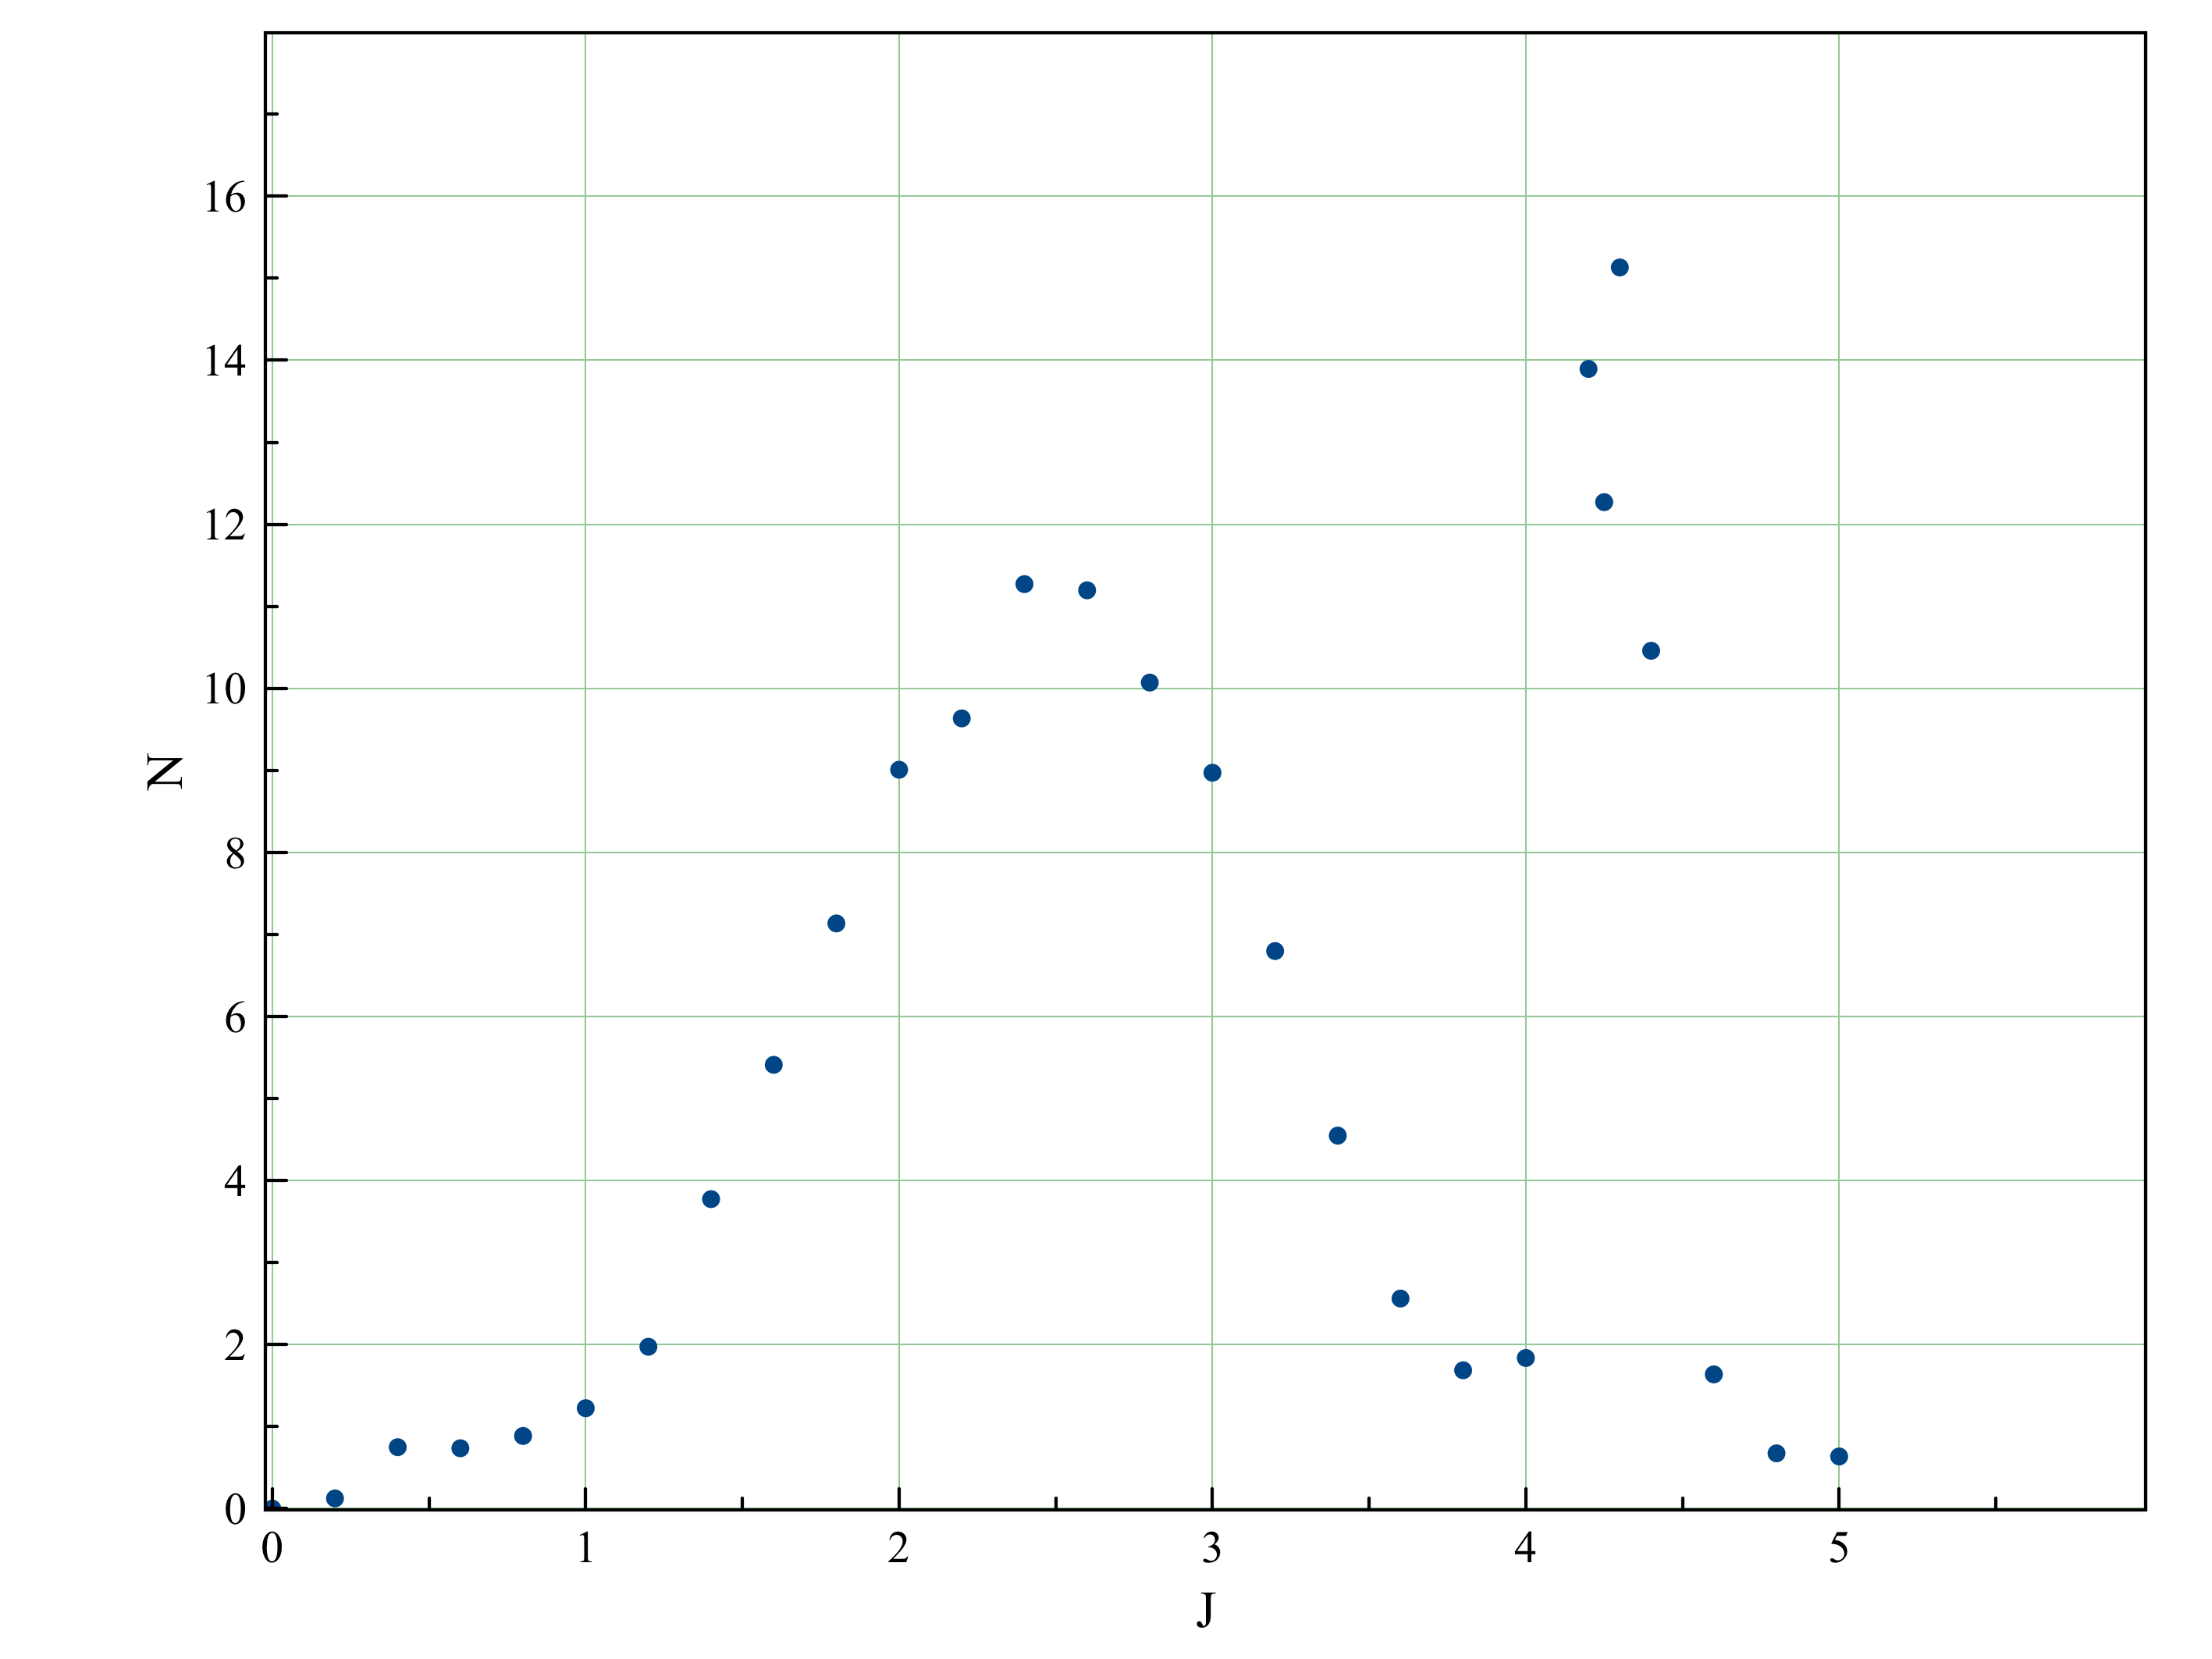
\includegraphics[width=\linewidth]{1.png}
	\caption{Форма спектра $\beta$-частиц при разрешенных переходах}
\end{figure}

\begin{figure}[h]
			\centering
			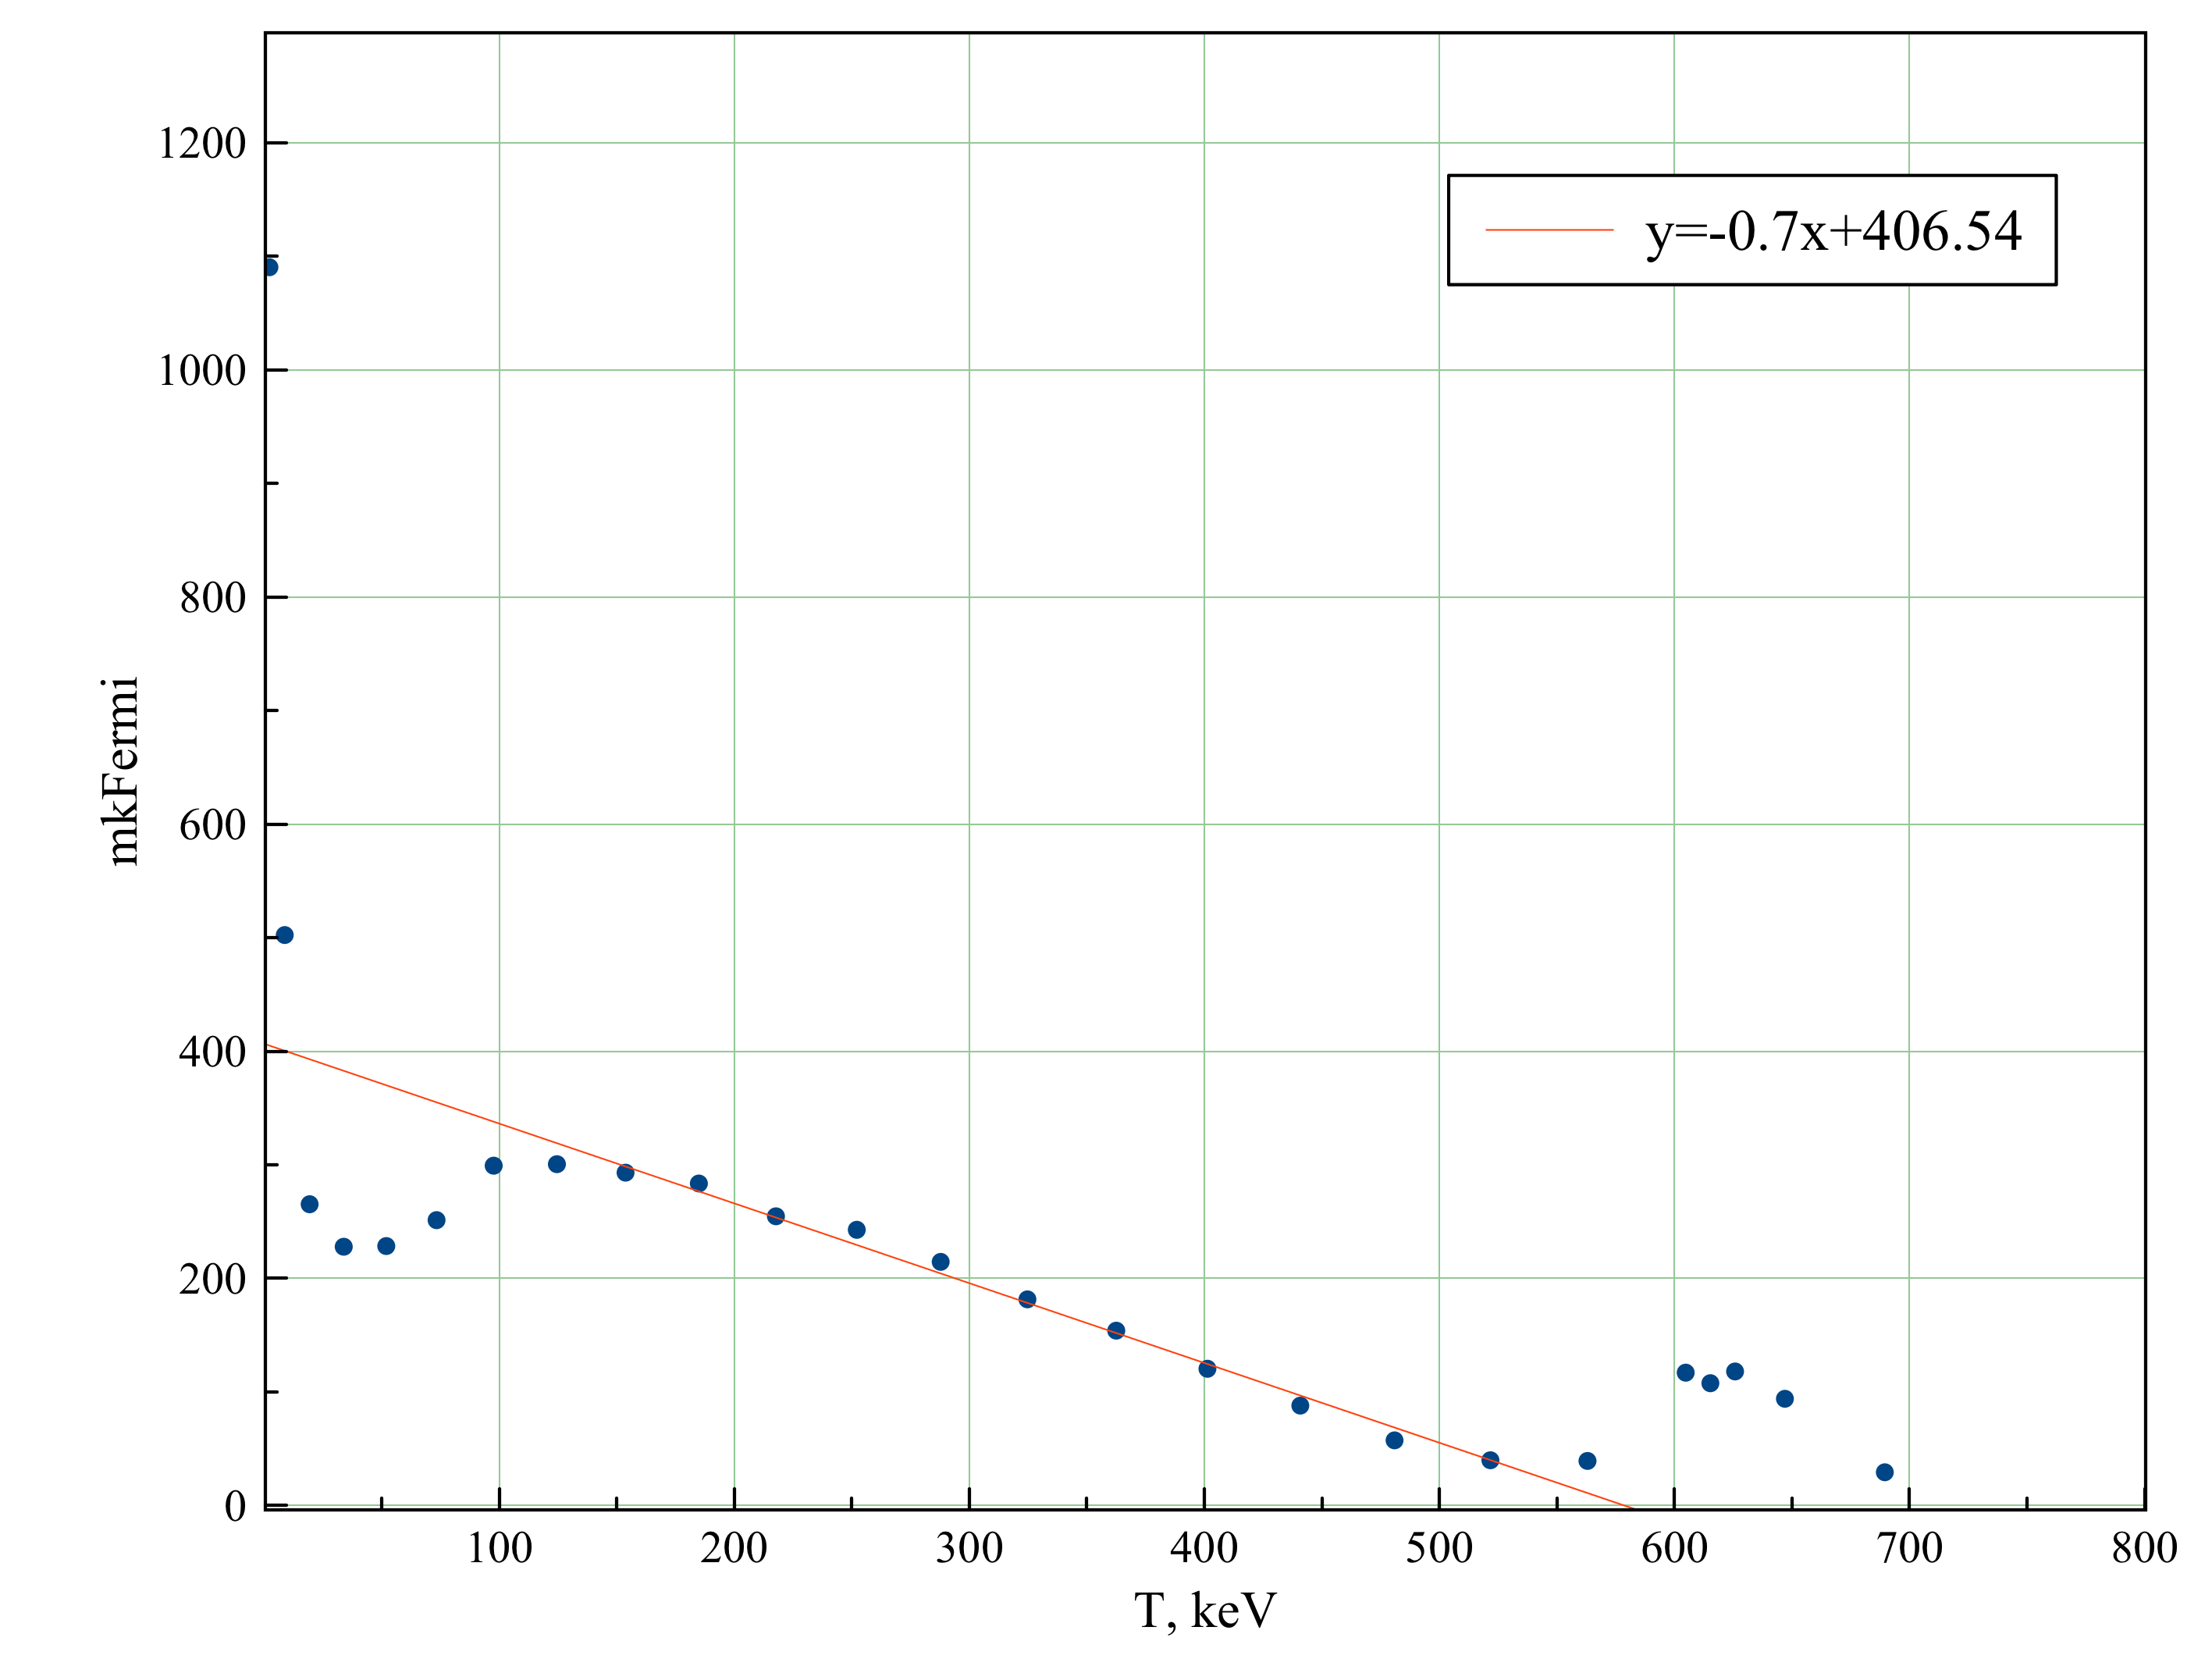
\includegraphics[width=\linewidth]{2.png}
			\caption{График Ферми-Кюри}
		\end{figure}
		
		
По точке пересечения графика с осью абсцисс определим максимальную энергию электронов в $\beta$-спектре. 
$E_{max} = 580.77 kEv$

\newpage

\section{Вывод и обсуждение результатов}
		В проделанной работе было исследовано явление $\beta$-распада $^{137}Cs$. Выявлен <<полудискретный>> характер спектра: непрерывная часть обеспечивается за счет рождения двух частиц, дискретный пик --- рождение конверсионных электронов.
		Непрерывность спектра доказывает существование антинейтрино и его рождение в процессе $\beta^-$ распада. Также было выяснено существование конверсионных электронов --- частиц, испускаемых в результате перехода ядра на более низкий энергетический уровень. Их энергетический спектр является уже дискретным, т.к. их энергия строго привязана к энергиям электронных уровней в атоме.
		Также была определена максимальная энергия электронов в $\beta$-спектре:
		$E_{max} = 580.77 kEv$
\end{document}


